\newcommand{\institut}{Institut f\"ur Telekommunikationssysteme}
\newcommand{\fachgebiet}{Nachrichten\"ubertragung}
\newcommand{\veranstaltung}{Praktikum Nachrichten\"ubertragung}
\newcommand{\pdfautor}{Dirk Babendererde (321 836), Thomas Kapa (325 219)}
\newcommand{\autor}{Dirk Babendererde (321 836)\\ Thomas Kapa (325 219)}
\newcommand{\gruppe}{Gruppe:}
\newcommand{\betreuer}{Betreuer: Lieven Lange}


\newcommand{\pdftitle}{Nachrichtenuebertragung\ Praktikum\ 05}
\newcommand{\prototitle}{Praktikum 05 \\ Pulsamplitudenmodulation und nichtideale Abtastung}

\input{../../packages/tu_header_9}

% damit das outline funktioniert noch mal:
\begin{document}


%     \lstinputlisting{./praktikum6.sce}

%---------------------------------------------------------------------
%---------------------------------------------------------------------
%---------------------------------------------------------------------

\section{Vorbereitung}
\begin{quote}
    
    
    \begin{figure}[H]
        \centering
        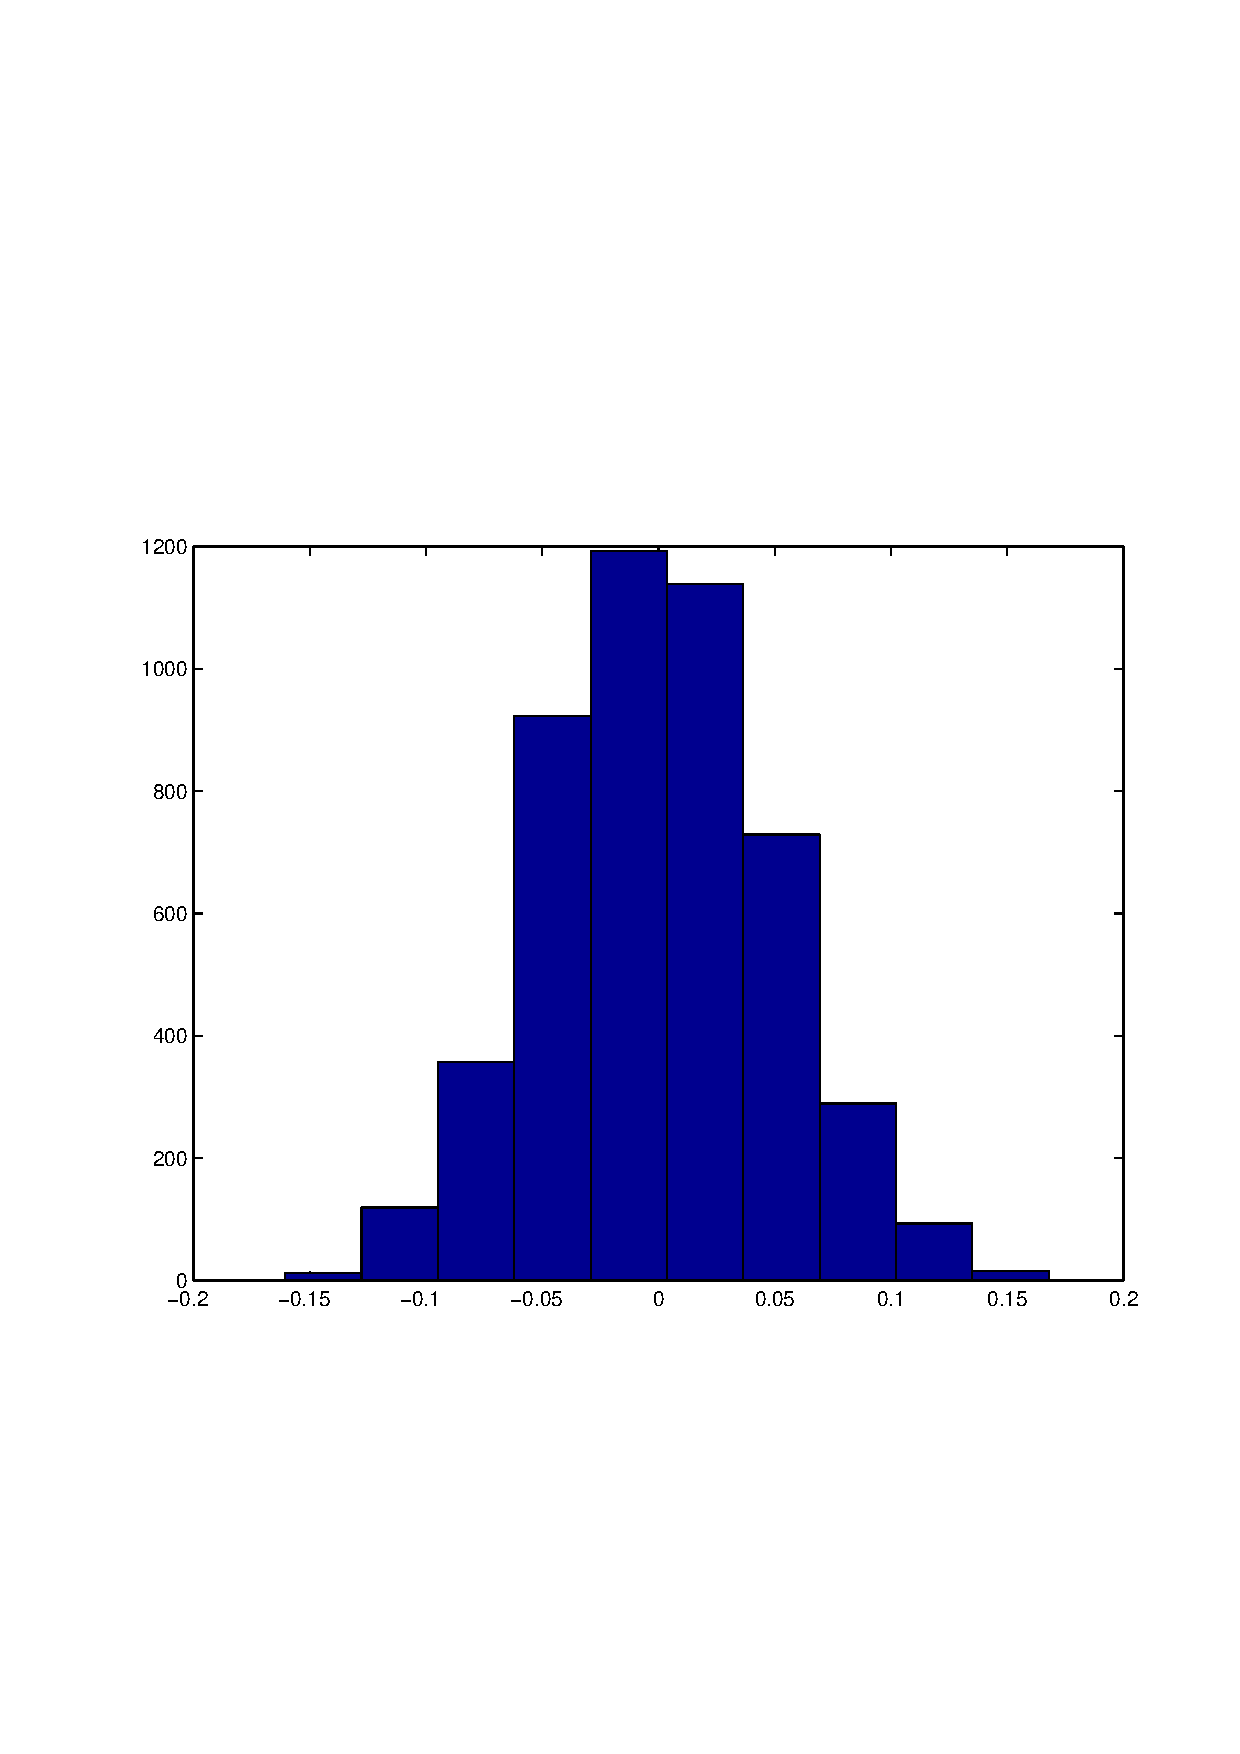
\includegraphics[scale=0.7, trim = 2cm 7cm 1cm 8cm, clip]{Bilder/PCM_Test}
        \caption{Testkennlinie des PCM-Analyse Scriptes}
        \label{fig:PCM_Test}
    \end{figure}
    
    
    \TODO{Blockschaltbild? erklärung?}
    
    
    
    
\end{quote}




\section{Auswertunf \& Theorie}
\begin{quote}
    
\end{quote}






\end{document}